% !TeX spellcheck = cs_CZ
{\tikzset{external/prefix={tikz/TKY/}}
 \tikzset{external/figure name/.add={ch02_}{}}
%============ Kapitola: Číslicové signály - posloupnosti ===========================================
\chapter{Číslicové signály - posloupnosti}
\minitoc

  Číslicové signály (matematicky posloupnosti čísel) \cite{Sovka} jsou v literatuře
  oz\-na\-čo\-vá\-ny symboly $x_n, x(n)$, nebo $x[nT]$, kde $n$ je celé číslo a označuje pořadí
  prvku v posloupnosti\footnote{Takto zavedené označení je nejednoznačné, neboť nerozlišuje mezi
  celou posloupností a jejím jediným prvkem. Posloupnost by měla být správně označena např.
  symbolem $\{x[n]\}$, zatímco symbol $x[n]$ by měl být vyhrazen pro její jeden prvek. Nicméně
  uvedené značení je všeobecně používáno.} Poslední uvedený symbol $x[nT]$ zdůrazňuje souvislost
  číslicového signálu se signálem spojitým v čase(analogovým signálem), ze kterého vznikl
  vzorkováním a kvantováním. Symbol $T$ označuje použitý \emph{vzorkovací krok}. Jeho převrácená
  hodnota je rovna \emph{vzorkovací frekvenci} $f_s=\frac{1}{T}$.

  \section{Základní typy posloupností}
    \begin{itemize}
      \item \textbf{Jednotkový impuls}
            \begin{equation}\label{SAS:eq_jednotkovy_imp}
              \delta[n]=
              \begin{cases} 
                 1, &  n = 0, \\
                 0, &  n \neq 0,
              \end{cases}
            \end{equation}
      \item \textbf{Jednotkový skok}
            \begin{equation}\label{SAS:eq_jednotkovy_skok}
              u[n]=
              \begin{cases} 
                 1, &  n \geq 0, \\
                 0, &  n < 0,
              \end{cases}
            \end{equation}
      \item \textbf{Reálná exponenciální posloupnost}
            \begin{equation}\label{SAS:eq_exp}
              x[n] = A\alpha^n, n\geq0,
            \end{equation}
      \item \textbf{Chirp signál}
            \begin{equation}\label{SAS:eq_chirp}
              x[n] = sin\left(\frac{\pi f_{max}n^2}{(N-1)f_s}\right),
            \end{equation}
            kde $f_{max}$ je maximální požadovaný kmitočet, který musí být menší než polovina
            vzorkovacího kmitočtu $f_{max}<\frac{f_s}{2}$ a $N$ je celkový počet vzorků.
      \item \textbf{Pseudonáhodná posloupnost} je posloupnost, která nahrazuje ideální bílý šum.
            Tuto posloupnost lze generovat různými algoritmy, které zaručují velmi dlouhou 
            periodicitu generované posloupnosti. Má-li tato posloupnost aproximovat bílý šum, musí 
            co nejlépe splňovat požadavek nekorelovanosti sousedních vzorků (tedy konstantní 
            spektrální výkonové hustoty) a nulové střední hodnoty. Často je požadován i jednotkový 
            rozptyl.
            \begin{figure}[ht!]
             \centering
             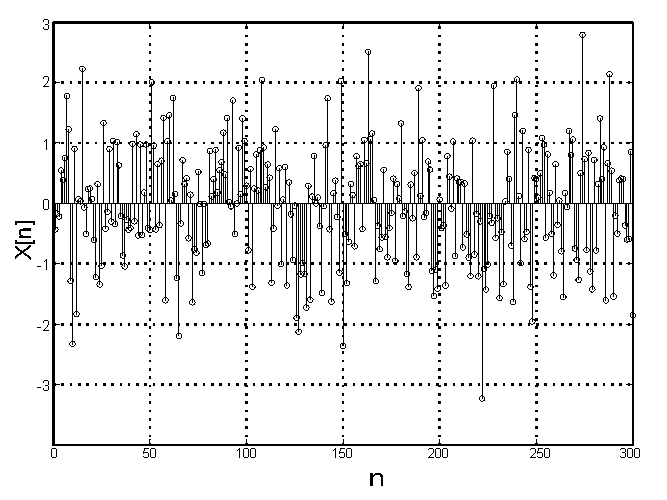
\includegraphics[width=0.8\linewidth]{randn_posloupnost.pdf}
             \caption[Příklad pseudonáhodné posloupnosti]{Příklad pseudonáhodné posloupnosti
                      generované pomocí funkce \texttt{randn(1, 300)} v MATLABu}
             \label{SAS:fig_randn}
         \end{figure}
    \end{itemize}
  
  \newpage
  \section{Generování jednoduchých signálů a jejich zobrazení v MATLABu}
    %---------------------------------------------------------------
    % !TeX spellcheck = cs_CZ Lineární obvody a systémy - Jan Bičák  - strana 10 Popis spojitých systémů
%===================================================================================================
\begin{mdframed}[style=mdexam]
  \begin{example}\label{tky:exam001}
    Uvažujme LTI systém, popsaný svou impulzní odezvou: \(h[n] = \{0.45, 1.72, 0.62\}\). Na jeho
    vstupu působí posloupnost \(x[n] = \{2,  0.95\}\). Úkolem  je vypočítat vzorky výstupní
    posloupnosti \(y[n]\).

    \noindent\textbf{Řešení:} Podle (\ref{tky:eq025}) bude délka výstupní posloupnosti \(N_y = 2 + 3
    - 1= 4\) s pořadovými indexy 0 až 3. Pro její výpočet rozepíšeme vztah (\ref{tky:eq024}):
    \begin{align*}
      y[0] &= \sum_{k=0}^0 x[0]h[0] = \num{2}\cdot\num{0.45} = \num{0.9}                   \\
      y[1] &= \sum_{k=0}^1 x[k]h[1-k] = x[0]h[1] + x[1]h[0] =                              \\
           &=  \num{2}\cdot\num{1.72} + \num{0.95}\cdot\num{0.45} = \num{3.8675}           \\
      y[2] &= \sum_{k=0}^2 x[k]h[2-k] =                                                    \\
           &= x[0]h[2] + x[1]h[1] + x[2]h[0] =                                             \\
           &= \num{2}\cdot\num{0.62} + \num{0.95}\cdot\num{1.72} + \num{0}\cdot\num{0.45}  
            = \num{2.8740}                                                                 \\
      y[3] &= \sum_{k=0}^3 x[k]h[3-k] =                                                    \\
           &= x[0]h[3] + x[1]h[2] + x[2]h[1] +  x[3]h[0] =                                 \\
           &= \num{2}\cdot\num{0} + \num{0.95}\cdot\num{0.62} + \num{0}\cdot\num{1.72}
            + \num{0}\cdot\num{0.45} =                                                     \\
           &= \num{0.589} 
    \end{align*} 
    Pro výstupní posloupnost tedy platí:
    \begin{equation*}
      y[n] = \{\num{0.9}, \num{3.8675}, \num{2.8740}, \num{0.589}\}
    \end{equation*}
    Situaci názorně shrnuje obr. \ref{tky:fig011}

    {\centering
      \captionsetup{type=figure}
      \luafigure[1]{tky_fig011.pdf}
      \captionof{figure}{Odezva lineárního číslicového systému na vstupní posloupnost. 
                \cite{Zaplatilek2013}}
      \label{tky:fig011}
    \par}

    V systému \textsc{MATLAB} je vestavěna vnitřní funkce \lstinline[style=luaMatlabText]!conv! pro
    snadný výpočet lineární diskrétní konvoluce, jak dokumentuje výpis \ref{tky:lst001}. Vyzkoušejme
    si, že obrátíme-li pořadí proměnných v příkazu \lstinline[style=luaMatlabText]!conv!, vyjde
    shodný výsledek (komutace symbolů).
  \end{example} 
  \begin{lstlisting}[style=luaMatlabText,gobble=4, label={tky:lst001}]
    h = [0.45, 1.72, 0.62];
    x = [2,  0.95];
    y = conv(x,h)
  \end{lstlisting}

\end{mdframed}
    %---------------------------------------------------------------

  \section{Základní operace s posloupnosti}
    V dalším textu budeme používat tři základní lineární operace \cite{Sovka} zobrazené na
    \ref{sas:fig_zakladni_operace}:
    \begin{itemize}
      \item \texttt{součin} signálu $x[n]$ a reálné konstanty $b$:      
            $$w[n]=bx[n], n = 0,1,2, \ldots$$ Tato operace je v praxi realizována násobičkou a je
            zdrojem numerických chyb, tedy kvantizačního šumu, který produkují číslicová zařízení.
      \item \texttt{součet} signálu $x[n]$ a signálu $y[n]$:           
            $$v[n]=x[n]+y[n], n = 0,1,2, \ldots$$ Tuto operaci provádí sčítačka. Při neošetření může
            tato operace generovat hrubé chyby.
      \item \texttt{zpoždění} signálu $x[n]$ o $k$ vzorkovacích kroků:  
            $$y[n]=x[n-k], n = 0,1,2, \ldots, n = 1,2, \ldots, M $$  Hodnoty $x[-k], k = 1, 2,
            \ldots, M$ se nazývají \emph{počáteční podmínky}. V digitálních implementací provádíme
            operaci zpoždění paměťového registru pro každou jednotku požadovaného zpoždění $z^{-1}$.
    \end{itemize}

    \begin{figure}[ht!]
      \centering
      \begin{tabular}{c}
        \hspace{0.1cm}
        \subfloat[ ]   {
          \begin{tikzpicture}[scale=1,>=latex']
  \coordinate (A) at (-1,-1.5) {};
  \coordinate (B) at (-1,-2.5) {};
  \coordinate (C) at (0,-2) {};    
  \coordinate (D) at ($ (A)!0.5!(B) $) {};
    \fill[fill=blue!20!white, draw=blue!50!black, very thick] (A) -- (B) -- (C) -- (A);
    \node[] at ($ (D)!0.4!(C) $) {\(b\)};
    \draw[->] (C) ++ (-2,0)  node[left] {\(x[n]\)} -- (D);
    \draw[->] (C) -+ (1,-2) node[right] {\(bx[n]\)}; 
\end{tikzpicture}}  \\
        \subfloat[ ]   {
          \begin{tikzpicture}[scale=1,>=latex']
  \coordinate (A) at (0,0) {};
  \coordinate (B) at (1,-1) {};   
  \coordinate (C) at ($ (A)!0.5!(B) $) {};   
  \coordinate (D) at (A |- C) {}; 
    \fill[fill=blue!20!white, draw=blue!50!black, very thick] (A) circle (0.5);
    \node[] at (A) {\(+\)};
    \draw[->] (-1.5,0) node[left] {\(x[n]\)} -- (-0.5,0);
    \draw[->] (0,1.5) node[above] {\(y[n]\)} -- (0,0.5);
    \draw[->] (0.5,0) --+ (1,0) node[right] {\(x[n]+y[n]\)}; 
\end{tikzpicture}
}  \\
        \subfloat[ ]   {
          \begin{tikzpicture}[scale=1,>=latex']
  \coordinate (A) at (0,0) {};
  \coordinate (B) at (1,-1) {};   
  \coordinate (C) at ($ (A)!0.5!(B) $) {};   
  \coordinate (D) at (A |- C) {}; 
    \fill[fill=blue!20!white, draw=blue!50!black, very thick] (A) rectangle (B);
    \node[] at (C) {\(z^{-k}\)};
    \draw[->] (D) + (-1,0) node[left] {\(x[n]\)} -- (D);
    \draw[->] (D) ++(1,0) --+ (1,0) node[right] {\(x[n-k]\)}; 
\end{tikzpicture}}    
      \end{tabular}
      \caption[Základní operace]{Symboly základních operací} 
      \label{sas:fig_zakladni_operace} 
    \end{figure}    

} %tikzset
%~~~~~~~~~~~~~~~~~~~~~~~~~~~~~~~~~~~~~~~~~~~~~~~~~~~~~~~~~~~~~~~~~~~~~~~~~~~~~~~~~~~~~~~~~~~~~~~~~~
\printbibliography[title={Seznam literatury}, heading=subbibliography]
\addcontentsline{toc}{section}{Seznam literatury}